\chapter{Experiments}
\label{chap:exp}

The fourth chapter presents our experiments and is split into two cases: one for the initial \acrshort{das} data loading and processing, where we use Judas, and one for training autoencoders and detecting anomalies using TinyDAS. Both follow a consistent structure: we begin with a detailed description of the dataset, followed by an explanation of the research methodologies. We then justify our choice of evaluation metrics and outline the experimental setups.
\section{Experiment 1: BANENOR}


\subsection{Dataset}


Our first experiment revolves around a \acrshort{das} dataset on a a train route between Trondheim and Storen, and is owned by BANENOR. The dataset spans the entirety of the 31st of August 2021\footnote{Working with national infrastructure requires security clearance, see \ref{app:conf} for more details}. The full route between Trondheim and Storen can be seen in appendix \ref{app:judas}. All the data is stored in hdf5 files.

\begin{table}[!htbp]
    \centering
    \small
    \begin{tabular}{@{}p{0.3\textwidth}p{0.4\textwidth}@{}}
        \toprule
        \textbf{Parameter} & \textbf{Value} \\
        \midrule
        Experiment & 210830\_NTNU\_Bane\_NOR\_GL8De4F2000  \\
        File timestamp & 2021-08-31 10:00:01  \\
        Type of data & Phase rate per distance (rad/m/s) \\
        Sampling frequency & \qty{2000}{\si{\hertz}} \\
        Window duration & \qty{10}{\si{\second}} \\
        Channel distance & \qty{4.0852}{\si{\meter}} \\
        \midrule
        Data shape & 20000 samples \(\times\) 12500 channels  \\
        \midrule
        Gauge length & \qty{8.1704}{ \si{\meter}} \\
        Sensitivities & \qty{9.3622e6}{\si{\radian}
        }\\
        Regions of interest (ROI) & 1:4:49996 \\
        \bottomrule
    \end{tabular}
    \caption{BANENOR Experiment Data Summary}
    \label{tab:experiment_data}
\end{table}


As we can see in table \ref{tab:experiment_data}, the total distance of this dataset is approximately 50km, where data from every 4th sensor across the route is stored. Each file contains 10 seconds of data, storing a $20000 \times 12500$ alongside relevant metadata, where each element is of type \texttt{Float32}, giving us a total of \qty{8}{\giga\byte} to be stored for every 10 seconds.  \\

\subsection{Evaluation}

In order to evaluate the improvements and additions to this package, we will be performing benchmarks both on individual functions, looking at the overall runtime of a realistic use-case.  
\paragraph{Parallel Resample function}We compare the parallel resampling method to a serial approach. Our input matrix will be a 5 minute DAS dataframe, with an effective ROI of [1:124:12499] giving an effective channel distance of \qty{200}{\si{\meter}}. The benchmark code can be found in.

\paragraph{Loading and Processing \acrshort{das} data}A full test from start to finish will be conducted. The experiment code can be found in \ref{app:judas}.

For both of these tests, speedups and parallel efficiency will be the main point of focus. We utilize different amounts of processes, and for the second benchmark, we compare


\subsection{Experiment Setup}

Due to national regulations, we will be performing all benchmarks on local servers belonging to \acrshort{cgf}. The system specifications can are all listed in the table below. \\


\begin{table}[htbp]
\centering
\begin{tabular}{@{}lll@{}}
\toprule
\textbf{Component} & \textbf{Specification} & \textbf{Details} \\
\midrule
Operating System & Ubuntu Linux & Version 20.04 LTS \\
Processor & Intel Core i9-9940X & \qty{4.40}{\giga\hertz} \\
RAM & 126 GB & DDR4-2400 MHz \\
GPU & NVIDIA GeForce RTX 2080 Ti &  \qty{11}{\giga\byte} GDDR6 \\
\bottomrule
\end{tabular}
\caption{System Specifications for Experimental Setup}
\label{tab:cgfsetup}
\end{table}
\clearpage
\section{Experiment 2: PUBDAS FORESEE}

\subsection{Dataset}

For this project, we will be using datasets from the PubDAS \cite{spica2023pubdas} collection. PubDAS is described as "A PUBlic Distributed Acoustic Sensing Datasets Repository for Geosciences" and contains \acrshort{das} data from numerous location all across the globe. We will specifically be dealing with the FORESEE dataset, a \acrshort{das} dataset stored in \acrshort{hdf5} files from an area around Pennsylvania in the Valley and Ridge Appalachians region  as seen in \ref{fig:foresee}. \\

\begin{figure}[!h]
    \centering
    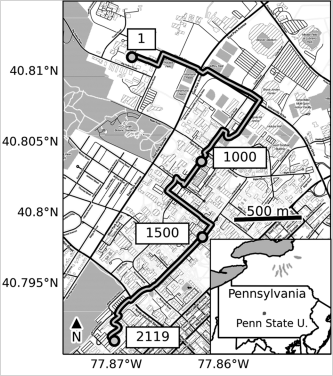
\includegraphics[width=0.5\linewidth]{figures/foresee.png}
    \caption{Map of the FORESEE Array. Photo is taken the PubDAS paper \cite{spica2023pubdas}}
    \label{fig:foresee}
\end{figure}

\begin{table}[!htbp]
    \centering
    \small
    \begin{tabular}{@{}p{0.3\textwidth}p{0.4\textwidth}p{0.2\textwidth}@{}}
        \toprule
        \textbf{Parameter} & \textbf{Value} & \textbf{Unit} \\
        \midrule
        Experiment & Foresee & \\
        Interrogator Unit (IU) & Silixa iDAS-v2 & \\
        Gauge length & 10 & \si{\meter} \\
        Cable length & 23300 & \si{\meter} \\
        Channel spacing & 2 & \si{\meter} \\
        \midrule
        \textbf{Original Data} & & \\
        Format & TDMS & \\
        Samples per second & 500 & \si{\hertz} \\
        File duration & 10 & \si{\minute} \\
        Data shape & 300000 \(\times\) 2137 & \\
        \midrule
        \textbf{After Preprocessing} & & \\
        Format & HDF5 & \\
        Samples per second & 125 & \si{\hertz} \\
        File duration & 5 & \si{\second} \\
        Data shape & 625 \(\times\) 2137 & \\
        \midrule
        \textbf{Dataset Information} & & \\
        Train dataset size & 25690 files & \\
        Train dataset span & 02 Mar 2020 08:10:15 to \newline 03 Mar 2020 20:40:10 & \\
        Labeled dataset size & 600 files & \\
        Labeled dataset span & 15 Apr 2019 03:17:35 to \newline 15 Apr 2019 04:07:30 & \\
        \bottomrule
    \end{tabular}
    \caption{FORESEE Experiment Data Summary}
    \label{tab:foresee_experiment_data}
\end{table}

PubDAS consist of 8 datasets stored in 3 different file formats. These 3 are \texttt{TDMS}, \texttt{HDF5} and \texttt{SEG-Y}. 
The FORESEE

\subsection{Data Preprocessing}

Some preprocessing on the dataset has already been done. This code is highlighted in the appendix \ref{app:pubdas}. To reduce the memory requirements of training such a dataset, we split the files into 5 second intervals compared to the original 10 minutes. Not only does this reduce memory requirements, but anomaly detection may be run every 5 seconds compared to the original 10 minutes. \\

Subsequentially, we chose a test dataset to label anomalies on based on this paper \cite{zhu2023seismic}, that found 18 thunder-induced seismic events in in this timestamp. We manually these data to be able to calculate confusion matrices and other relevant metrics to test the accuracy of our autoencoders. Information about these datasets can be found in table \ref{tab:foresee_experiment_data}. \\

When first downloading these data, they're stored in 10-minute files, resulting in quite large files as shown below:

\begin{align*}
\text{Size} &= 10 \times 60 \times 125 \times 2137 \times 4 \\
&= 600 \times 125 \times 2137 \times 4 \\
&= 641,100,000 \text{ bytes} \\
&\approx 641.1 \text{ MB} \\
&\approx 0.6411 \text{ GB}
\end{align*}

where:
\begin{itemize}
    \item 10 minutes is the duration of each file
    \item 60 seconds per minute
    \item 125\si{\hertz} is the sampling rate
    \item 2137 is the number of channels
    \item 4 bytes per sample (Float32)
\end{itemize}

Most consumer grade \acrshort{gpu}s can only store about 8-16gb of data in VRAM, thus meaning the batches of data we can store is not that big. Additionally, not only does the \acrshort{gpu}s have to store data, but also the weights and biases of the model, as well as losses and more. Motivated by this, we decide to split the files to last 5 seconds compared to 10 minutes. \\ 

We start of by looking at the file names and removing the prefix \textbf{FORESEE\_UTC\_}, since we're only working with one dataset at the time. Furthermore, in parallel fashion, we split each of the files in smaller ones, calculating new filenames based on the beginning timestamp. Now, each \acrshort{hdf5} file store a $625*2137$ matrix of \acrshort{das} data, successfully reducing the memory usage. 
These data are originally stored as \texttt{Float32}, but will be casted as \texttt{Float16} for faster training as we will see later on. In total, more than 25 000 files from the month of april 2020 is gathered to train our model on. 
RESULT: SPEAK ABOUT 5 SECONDS FOR LIVE ENVIRONMENT.
TODO: Inference data from 15042019!


\subsection{Evaluation}

We will be separating the evaluation of \texttt{TinyDAS} into two sections. The first section will focus more on overall model training. Here is a list of points to be evaluated: 

\begin{itemize}
    \item \textbf{Experiment 1}: Median training time and model sizes, and losses
    \item \textbf{Experiment 2}: Reconstruction Capabilities
\end{itemize}

The second section will revolve around anomaly detection based on the different architectures. There are several different methods to evaluate the effectiveness and accuracy of models designed for anomaly detection. A very common pattern is to measure predicted results up against some ground truths, and construct a confusion matrix based on the result. As we saw in listing \ref{code:thresh}. To be able to evaluate the model, we first label ground truths. This is done by iterating over files in a dataset, marking indices of anomalous data to a text file. Furthermore, we will be constructing a confusion 

From this confusion matrix, the following metrics will be used. \\ 


The True Positive Rate (TPR), also known as recall calculated the percentage of truths calculated out of all ground truths. TP is true positives, and FN is false negatives. 

\begin{equation}
    TPR = \frac{TP}{TP + FN} = Recall
\end{equation}
\vspace{0.2cm}

Likewise, the False Positive Rate is the percentage of falsehoolds calculated out of all the ground negatives. FP is false negatives, and TN is true negatives:

\begin{equation}
    FPR = \frac{FP}{FP + TN}
\end{equation}
\vspace{0.2cm}

Precision is the percentage of correct truths out of all predicted truths.

\begin{equation}
    Precision = \frac{TP}{TP + FP}
\end{equation}

\vspace{0.2cm}

The $F1\_{score}$ is used to evaluate the balance between intrusion detection accuracy and recall rate; the higher the score, the better:
\begin{equation}
    F1\_{score} = 2 \times (\frac{Precision \cdot Recall}{Precision + Recall})
\end{equation}

\vspace{0.2cm}

Accuracy measures the proportion of correct predictions:

\begin{equation}
    Accuracy = \frac{TP + TN}{TP + TN + FP + FN}
\end{equation}

\vspace{0.5cm}

For the anomaly detection part of TinyDAS, the following experiments will be conducted

\begin{itemize}
    \item \textbf{Experiment 4}: Anomaly Detection Accuracy
    \item \textbf{Experiment 5}: Confusion Matrix and Metrics
\end{itemize}


\subsection{Experiment Setup}

All the models were trained and tested on \gls{idun} computers made for \acrshort{hpc}. Configuration parameter for the different models can be found in the appendix \ref{app:judasnethyperparams}, and details of the machines used can be found in the table below. \\


\begin{table}[!htbp]
\centering
\caption{Specifications for Model Training and Testing Environment}
\label{tab:system-specs}
\begin{tabular}{@{}llr@{}}
\toprule
\textbf{Component} & \textbf{Description} & \textbf{Quantity} \\
\midrule
Operating System & Ubuntu Linux 22.04 LTS & 1 machine \\
GPU Model & NVIDIA H100 PCIe & 4 units \\
GPU Memory & HBM3 & 80 GB per GPU \\
CUDA Cores & & 14,592 per GPU \\
Tensor Cores & & 576 per GPU \\
GPU Clock Speed & Boost Clock & 1.67 GHz \\
GPU TDP & & 350 W \\
FP16 & & 204.9 TFLOPS \\
FP32 & & 51.22 TFLOPS \\
\midrule
\multicolumn{3}{@{}l@{}}{\textit{Note:} 1 \acrshort{gpu} dedicated for testing, 4 for training.} \\
\bottomrule
\end{tabular}
\end{table}


